% Chapter of Volume III: Approximating Xi by laws with real zeros. Sources: misc/reviews/nick-approx/approx_chapter/approx_chapter.tex lines 35-339 (draft, Polson, November 2026); report APPROX (misc/research/directions/opus/vol3/APPROX.md, M1 to M9); verification misc/vol3/verify/APPROX/results.md; 17 Nov 2026.
\label{ap:ch:approx}

By Hurwitz's theorem, RH would follow from a sequence of functions with only real zeros that converges locally uniformly to $\Xi(t)=\xi(\frac12+it)$. This chapter studies that idea in probabilistic form, with the laws of Volume II as the approximants. The characteristic function $\Xi(t)/\Xi(0)$ belongs to a law $V$, a tilted logarithm of the variable of Biane, Pitman and Yor \cite{BPY01}. Section~\ref{ap:sec:law} places $V$ next to its Wald partner and its van Dantzig partner, which Chapter~\ref{c:ch:cand} established. Section~\ref{ap:sec:factor} proves that one real zero can be divided out of $\Xi$ and still leave a characteristic function, and reports numerical evidence that the zeros of $\Xi$ can be split into two halves that are characteristic functions. Section~\ref{ap:sec:gig} fits products of symmetrised generalised inverse Gaussian (GIG) characteristic functions to $\Xi$ on windows and shows that each factor follows only two or three zeros of $\zeta$. Section~\ref{ap:sec:closure} proves what the limits of such products are. The consequence is a reduction, and nothing more: $\Xi/\Xi(0)$ is such a limit only if RH holds and the ordinates of the zeros are a disjoint union of complete zero sets of members of a closure that we describe in part. We expect that they are not, which would close this route to RH. That expectation rests on an open problem (Problem~\ref{ap:prob:notG}), so it is a heuristic and not a theorem.

\section{The law \texorpdfstring{$V$}{V} and its partners}\label{ap:sec:law}

With $\Phi(x)=2\sum_{n\ge1}(2\pi^2n^4e^{9x/2}-3\pi n^2e^{5x/2})\exp(-\pi n^2e^{2x})$, Riemann's formula is $\Xi(t)=\int_{\mathbb R}\Phi(x)\cos(tx)\,\mathrm dx$. The function $\Phi$ is positive, even and decreasing on $(0,\infty)$, a classical fact due to Wintner, so $f=\Phi/\Xi(0)$, with $\Xi(0)=0.4971207782$, is a probability density. Let $V$ have density $f$. Let $Y=\sqrt{(\pi/2)(T+T')}$ be the variable of Biane, Pitman and Yor, with $\mathbb E\,Y^s=2\xi(s)$, where $T,T'$ are independent hitting times of level $1$ by a three dimensional Bessel process. Then $V$ is $\log Y$ under the law of $Y$ tilted by $y^{1/2}$, because $\mathbb E\,e^{\theta V}=\xi(\frac12+\theta)/\xi(\frac12)$.

The variance of $V$ is $(\log\xi)''(\frac12)=0.04620998623$ (computed), the constant $V_\xi$ of Section~\ref{dz:sec:comp}, and $\kappa_4(V)=-4.46071\times10^{-4}$ (computed). Under RH, $\Xi(t)/\Xi(0)=\prod_{\gamma>0}(1-t^2/\gamma^2)$ and the cumulants are power sums of the ordinates,
\[
\kappa_{2k}(V)=(-1)^{k+1}\frac{(2k)!}{k}\sum_{\gamma>0}\gamma^{-2k},
\]
so that $\mathrm{Var}(V)=2\sum\gamma^{-2}$ and $\kappa_4=-12\sum\gamma^{-4}$. Both values were computed from $\xi''/\xi$ and from the zeros. The law $V$ is not infinitely divisible, without any hypothesis, because its characteristic function has real zeros.

We use the Wald couple of Proposition~\ref{c:thm:wald} without change. Its first item is unconditional: $V$ has a Wald partner $H$, with $\mathbb E\,e^{\theta V}\,\mathbb E\,e^{-\theta^2H/2}=1$. Its second item says that RH holds if and only if $H$ is a generalised gamma convolution, and then $H=\sum_{\gamma>0}\mathrm{Exp}(\gamma^2/2)$, with Thorin measure $\sum_{\gamma>0}\delta_{\gamma^2/2}$. Here $H=2T$ for the clock variable $T$ of Section~\ref{ch:clock}; this is the only place in the chapter where the normalisation of Chapter~\ref{c:ch:cand} matters, and all Thorin measures below are in the variable of $H$. Let $B_H$ denote Brownian motion run for the independent time $H$. Under RH,
\[
\frac{\Xi(t)}{\Xi(0)}\cdot\prod_{\gamma>0}\Big(1+\frac{(it)^2}{\gamma^2}\Big)^{-1}=1,
\]
and $\prod(1+t^2/\gamma^2)^{-1}=\mathbb E\,e^{-t^2H/2}$ is the characteristic function of $B_H$. So $V$ and $B_H$ form a van Dantzig pair in the sense of Lukacs \cite{Lukacs68}, and the three objects have the transforms $\prod(1-t^2/\gamma^2)$ for $V$, $\prod(1+2u/\gamma^2)^{-1}$ for $H$ at $e^{-uH}$, and $\prod(1+t^2/\gamma^2)^{-1}$ for $B_H$. The classical examples are the same pattern with other spectra: $\cos t$ with $1/\cosh t$, where $V=\pm1$ is the position of a Brownian motion at the exit time $H$ of $(-1,1)$ and $1/\cosh t$ is the characteristic function of the motion at an independent time $H$; $\sin t/t$ with $t/\sinh t$; and the normal law with itself, where $H$ is constant.

The identity behind the passage from the L\'evy side to the Thorin side is the sine squared lemma, which is equation~\eqref{eq:sin2} after the substitution $z\to z/2$: for $\theta\ge0$ and $x>0$, with $u=\theta^2/2$,
\[
e^{-\theta x}-1+\theta x=\int_0^\infty\log\Big(1+\frac uz\Big)\frac{x}{\pi\sqrt{2z}}\,2\sin^2\!\big(x\sqrt{z/2}\big)\,\mathrm dz .
\]
It is unconditional, and it is an identity for a single exponential. Integrating it against the L\'evy measure of $V$ gives the Thorin measure of $H$ only under a hypothesis. At rung $\frac12$ the measure $m$ in $\log\mathbb E\,e^{\theta V}=\int(e^{-\theta x}-1+\theta x)\,m(\mathrm dx)$, with atoms at logarithms of prime powers and a negative density from the pole, does not converge absolutely, since $\sum\Lambda(n)n^{-1/2}$ diverges. For $0<\theta<\frac12$ its convergence amounts to the absence of zeros with real part above $\frac12+\theta$. So we do not use a rung $\frac12$ form and no transfer criterion at that rung. The criterion of this book is Theorem~\ref{thm:dbeta:minall}(vi), over the rungs $\alpha\in(\frac12,1)$.

Sums of independent variables add Thorin measures on the side of $H$. A subset $S$ of the atoms gives a legitimate generalised gamma convolution $H_S=\sum_{\gamma\in S}\mathrm{Exp}(\gamma^2/2)$. On the side of $V$ the same subset gives $P_S(t)=\prod_{\gamma\in S}(1-t^2/\gamma^2)$, which may or may not be a characteristic function; a single factor $1-t^2/\gamma^2$ is not one. So products for $V$ correspond to sums for $H$ and to sums of Thorin measures, and splitting $V$ into independent pieces is splitting the measure $\sum\delta_{\gamma^2/2}$ into parts that each have a Wald partner. Problem~\ref{fm:prob:split} asks whether this is possible.

\section{Factors of \texorpdfstring{$V$}{V}}\label{ap:sec:factor}

\begin{proposition}[what a factor is]\label{ap:prop:factor}
Assume RH. Let $V=V_1+V_2$ with independent nondegenerate summands. Then up to a shift the characteristic function of $V_1$ is $P_S$ for a set $S$ of ordinates (counted with multiplicity) and that of $V_2$ is $P_{S^c}$. Each factor has only real zeros, and $S$, $S^c$ are both infinite. In Thorin terms $H=H_S+H_{S^c}$, a split of the centre measure in which both parts have Wald partners.
\end{proposition}

\begin{proof}
The variable $V$ is symmetric with $\mathbb E\,e^{sV}=\xi(\frac12+s)/\xi(\frac12)<\infty$ for all real $s$, and $\mathbb E V=0$. Shift the summands so that $\mathbb E V_1=\mathbb E V_2=0$. Then $\mathbb E\,e^{sV_i}\ge1$ by Jensen's inequality, so $\mathbb E\,e^{sV_1}\le\mathbb E\,e^{sV}$, and the same for $V_2$. Hence the characteristic functions $\varphi_i(z)=\mathbb E\,e^{izV_i}$ are entire, with $|\varphi_i(x+iy)|\le\mathbb E\,e^{|y||V_i|}\le\mathbb E\,e^{yV}+\mathbb E\,e^{-yV}$, and since $\xi$ has order $1$ they have order at most $1$. Every zero of $\varphi_i$ is a zero of $\varphi_1\varphi_2=\Xi/\Xi(0)$, so it is real, and the zero set of a characteristic function is symmetric under $t\mapsto-t$, because $\varphi(-t)=\overline{\varphi(t)}$. By Hadamard's theorem, $\varphi_i(t)=e^{c+\beta t}P_{S_i}(t)$ where $S_i$ is the set of positive zeros, the exponent has degree at most $1$, and $P_{S_i}$ converges because $\sum\gamma^{-2}<\infty$. Since $|\varphi_i|\le1$ on $\mathbb R$ and $\varphi_i(0)=1$, $c=0$ and $\beta$ is purely imaginary. The zeros multiply, so $S_1$ and $S_2$ split the ordinates. If $S_1$ were finite then $\varphi_1$ would be a polynomial bounded on $\mathbb R$, hence constant, and $V_1$ would be degenerate. This is also Theorem~\ref{fm:thm:nosqrt}.
\end{proof}

Proposition~\ref{ap:prop:factor} is the reduction already stated in Problem~\ref{fm:prob:split}, which also notes that under Ingham's hypothesis of linear independence of the ordinates over the rationals no piece can have an arithmetic progression among its zeros. What is new here is the next result, which says that a single zero can always be removed.

\begin{lemma}[removing a zero]\label{ap:lem:remove}
Let $f$ be an even probability density, nonincreasing on $(0,\infty)$, with characteristic function $\varphi$, and let $\varphi(\gamma)=0$ with $\gamma>0$. Then $\varphi(t)/(1-t^2/\gamma^2)$ is the characteristic function of the probability density
\[
q(x)=\gamma\int_0^\infty\sin(\gamma u)\,f(|x|+u)\,\mathrm du,\qquad0\le q(x)\le2f(x).
\]
\end{lemma}

\begin{proof}
Put $q_0(x)=\gamma\int_{-\infty}^x\sin(\gamma(x-y))f(y)\,\mathrm dy$. Differentiating twice gives $q_0''=\gamma^2(f-q_0)$. For $x<0$ the substitution $y=x-u$ and the evenness of $f$ turn $q_0$ into the stated integral. For $x>0$, the integral over all of $\mathbb R$ equals $\gamma\,\mathrm{Im}\big(e^{i\gamma x}\varphi(\gamma)\big)=0$, because $\varphi(\gamma)=0$, so $q_0(x)=\gamma\int_x^\infty\sin(\gamma(y-x))f(y)\,\mathrm dy$, which is the same formula. So $q_0=q$ is even. For fixed $x\ge0$ the function $u\mapsto f(x+u)$ is nonnegative and nonincreasing, so the integral of $\sin(\gamma u)f(x+u)$ over the successive half periods of $\sin(\gamma u)$ is an alternating series with decreasing terms. It lies between $0$ and its first term, which is at most $f(x)\int_0^{\pi/\gamma}\sin(\gamma u)\,\mathrm du=2f(x)/\gamma$. Hence $0\le q\le2f$, and $q$ is integrable. Fourier transformation of $q''/\gamma^2+q=f$ gives $(1-t^2/\gamma^2)\hat q(t)=\varphi(t)$, so $\hat q(0)=1$ and $q$ is a probability density with the stated transform.
\end{proof}

\begin{theorem}[removing a zero of $\Xi$]\label{ap:thm:remove}
For every real zero $\gamma$ of $\Xi$, the function $\Xi(t)/\big(\Xi(0)(1-t^2/\gamma^2)\big)$ is a characteristic function. This holds without any hypothesis.
\end{theorem}

\begin{proof}
Apply Lemma~\ref{ap:lem:remove} to $f=\Phi/\Xi(0)$, which is even and nonincreasing on $(0,\infty)$.
\end{proof}

For the first zero the density $q$ at $x=0$, $0.2$, $0.5$ is $2.0655$, $1.2215$, $0.0628$ (computed), by the lemma and by numerical inversion of the product. We have not found Theorem~\ref{ap:thm:remove} in the literature. It, the splitting computations and Theorem~\ref{ap:thm:closure} come from an unrefereed note of Polson (November 2026). In Thorin terms, one atom can always be taken out of the centre measure without losing the Wald partner of what is left. Lemma~\ref{ap:lem:remove} can be iterated only if $q$ is again nonincreasing on $(0,\infty)$. This holds on a grid of $x\in[0,3]$ of step $0.025$ for the first zero (computed), and it is open in general (Problem~\ref{ap:prob:iterate}).

\subsection{Splitting the zeros in half}\label{ap:sec:split}

We computed $P_S(t)$ for $0\le t\le260$ from the $1545$ zeros below height $2030$, and inverted it numerically. The products and the variances in Table~\ref{ap:tab:split} include the tail of the zeros beyond $2030$, which is shared among the sets in proportion to their density; the variances over the $1545$ zeros alone are smaller by $0.0004$ to $0.0011$. All entries are computed in double precision and not certified.
\begin{table}[t]
\centering
\small
\begin{tabular}{lcccc}
\toprule
set $S$ & $\sup|P_S|$ & variance & positive & decreasing\\
\midrule
odd indexed zeros & $1$ & $0.02685$ & yes & yes\\
even indexed zeros & $1$ & $0.01936$ & yes & yes\\
a random half & $1$ & $0.02977$ & yes & yes\\
two zeros in three & $1$ & $0.02592$ & yes & yes\\
every third zero & $1$ & $0.02029$ & yes & no, two modes\\
all but the first $100$ & $1$ & $0.00622$ & yes & yes\\
every tenth zero, offset $0$ & $1.20$ & & no & \\
every tenth zero, offsets $1$ to $9$ & $1.00$ & & no, barely & \\
random tenths (four draws) & & & three of four no & \\
\bottomrule
\end{tabular}
\caption{Subsets of the ordinates of $\zeta$ and the inverse transform of $P_S$ (computed). The variance of the random half is not independently checked. Offset $0$ means the zeros of indices $1,11,21,\dots$. For offsets $1$ to $9$ the minimum of the inverse transform is between $-7\times10^{-6}$ and $-3\times10^{-7}$.}\label{ap:tab:split}
\end{table}
% UNVERIFIED: variance 0.02977 of the random half (not in the verification list); all other rows reproduced by independent code.
So, numerically, $V\overset{d}{=}V_{\mathrm{odd}}+V_{\mathrm{even}}$ and $H=H_{\mathrm{odd}}+H_{\mathrm{even}}$ with both Wald couples in place. Every tenth zero fails for all ten offsets, for offset $0$ because $\sup|P_S|>1$ and for the other nine only by a negative minimum between $-7\cdot10^{-6}$ and $-3\cdot10^{-7}$. Of four random tenths three failed and one did not. So sets of proportion one tenth can fail, and a random one need not. Nothing here shows that a positive proportion is necessary, since a nondegenerate factor needs only positive exponential type, which a set of zero density can have.
\begin{figure}[t]
\centering
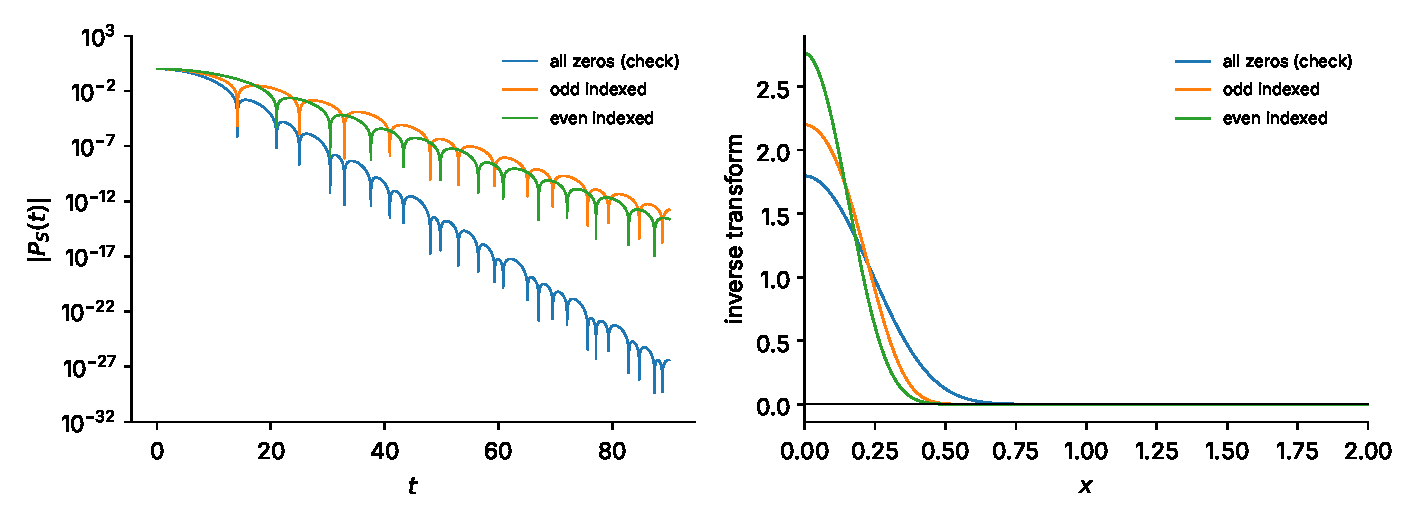
\includegraphics[width=\textwidth]{fig/v3/ap_splits.pdf}
\caption{Left: $|P_S(t)|$ for all zeros and for the odd and even indexed halves. Right: their inverse transforms, positive and decreasing on $x>0$ (computed).}\label{ap:fig:split}
\end{figure}
\begin{remark}[conjecture]\label{ap:rem:conj}
We conjecture that there is a proportion $\theta_0<\frac13$ such that for every set $S$ of ordinates that is spread out in proportion at least $\theta_0$, $P_S$ is a characteristic function. We cannot define the class of sets precisely, and the conjecture is open.
\end{remark}

\section{Products of inverse Gaussian laws}\label{ap:sec:gig}

Volume II already contains approximants of $\Xi$ with real zeros that are accurate on a window. The laws of Theorem~\ref{fm:thm:bessel} have real zeros by theorem and, for one kernel, a certified total variation distance below $6.1\times10^{-6}$ from the P\'olya law (Table~\ref{fm:tab:bessel}); the zero completed laws $f_K$ of Theorem~\ref{fm:thm:zc} have real zeros and keep the first $K$ zeros exactly, with certification for $K\le200$. The folded truncations of the kernel $\Phi$ are accurate up to the height of order $4(N+1)^2$ and then fail (Table~\ref{ev:tab:approx}), and P\'olya's own approximants and the heat flow are in Section~\ref{fm:sec:simple}. This section studies products of Theorem~\ref{fm:thm:bessel}'s laws, which is the case $J=0$ of Corollary~\ref{fm:cor:coupled}.

A symmetrised GIG component is $U=c\log W$, where $W$ has density proportional to $y^{\pm\nu-1}e^{-a(y+1/y)}$, with either sign of $\nu$ equally likely. Then
\[
\varphi_{c,\nu,a}(t)=\mathbb E\,e^{itU}=\frac{K_{\nu+ict}(2a)+K_{\nu-ict}(2a)}{2K_\nu(2a)} .
\]
In the notation of Theorem~\ref{fm:thm:bessel} and Proposition~\ref{fm:prop:besselgig} this is the law with kernel $e^{-a_{\mathrm{book}}\cosh\ell t}$, where $\ell=1/c$, $a_{\mathrm{book}}=2a$, $\mu=0$ and one field $\lambda_1=\nu\ell$, that is $m(t)=\cosh(\nu\ell t)$. It has only real zeros, by P\'olya's theorem \cite{Polya} and Theorem~\ref{fm:thm:bessel}(i). P\'olya's own approximant is the single component $c=\frac12$, $\nu=\frac94$, $a=\pi$. Let $\mathcal K$ be the set of all components.

We read the zero sets with care. For $\nu=0$ the zeros of $\varphi_{c,0,a}$ are $\tau_n/c$, where $K_{i\tau_n}(2a)=0$; since $K_{i\tau}(2ae^y)$ solves $-f''+4a^2e^{2y}f=\tau^2f$ on the half line, the numbers $\tau_n^2$ are the Dirichlet eigenvalues of the Schr\"odinger operator with exponential potential (see the proof of Theorem~\ref{fm:thm:bessel}). For instance $\tau_1=4.4255$ when $a=1$ (computed). For $\nu\ne0$ the zero set is the zero set of $z\mapsto K_{\nu+iz}(2a)+K_{\nu-iz}(2a)$ at $z=ct$. It is not $\{\tau_n/c\}$, and it is not a Dirichlet spectrum of that operator. Every fitted component below has $\nu$ between $0.52$ and $1.05$. By Corollary~\ref{fm:cor:coupled} at $J=0$ and Remark~\ref{fm:rem:besselcount} a product $\prod_j\varphi_{c_j,\nu_j,a_j}$ has the main term of the Riemann von Mangoldt count of $\Xi$ exactly when $\sum_jc_j=\frac12$ and a second, logarithmic condition on the $a_j$ holds. We test only the first.

\subsection{The fits}\label{ap:sec:fits}

Components were fitted by least squares to $\Xi(t)/\Xi(0)$ on a window $0\le t\le T$, with weight $e^{\pi t/4}(1+t)^{-7/4}$. Nothing was imposed on $\sum c_j$. The error in Table~\ref{ap:tab:fits} is the weighted root mean square residual.
\begin{table}[t]
\centering
\footnotesize
\setlength{\tabcolsep}{4pt}
\begin{tabular}{lcccl}
\toprule
fit & $T$ & $\sum c_j$ & error & zeros\\
\midrule
P\'olya, one component & $32$ & $0.5$ & $9.1$ & $8.99,\ 19.07,\ 24.47$\\
$1$ component & $32$ & $0.483$ & $0.99$ & $14.18,\ 20.86,\ 25.69$\\
$2$ components & $32$ & $0.487$ & $6\times10^{-4}$ & first $5$ to $0.001$\\
$3$ components & $32$ & $0.496$ & $1\times10^{-5}$ & first $5$ to $0.001$\\
$4$ components & $44$ & $0.495$ & $1\times10^{-4}$ & first $8$ to $0.001$\\
$5$ components & $44$ & $0.499$ & $1\times10^{-5}$ & first $8$ to $0.001$\\
\bottomrule
\end{tabular}
\caption{Least squares fits of products of $\mathcal K$ to $\Xi/\Xi(0)$ (computed in double precision, not certified). The first two rows and the four component row are reproduced by independent code (the refit of the four component row gives error $5\times10^{-5}$ and $\sum c_j=0.496$); the two, three and five component rows are not independently checked.}\label{ap:tab:fits}
\end{table}
% UNVERIFIED: rows with 2, 3 and 5 components of the fits table (parameters not printed in the draft).
The sums of the scales come out near $\frac12$ although nothing imposed it. The fits are flexible, with three parameters per component against about two zeros per component in the window, and they leave the window badly: a four component refit predicts the zero $48.005$ just outside the window as $48.02$ (computed), but the other zeros outside it are off by more, as Table~\ref{ap:tab:carry} shows. The fits are computed and not certified. They are not a statement about total variation; the certified bounds of this kind in the book are those of Table~\ref{fm:tab:bessel}.
\begin{figure}[t]
\centering
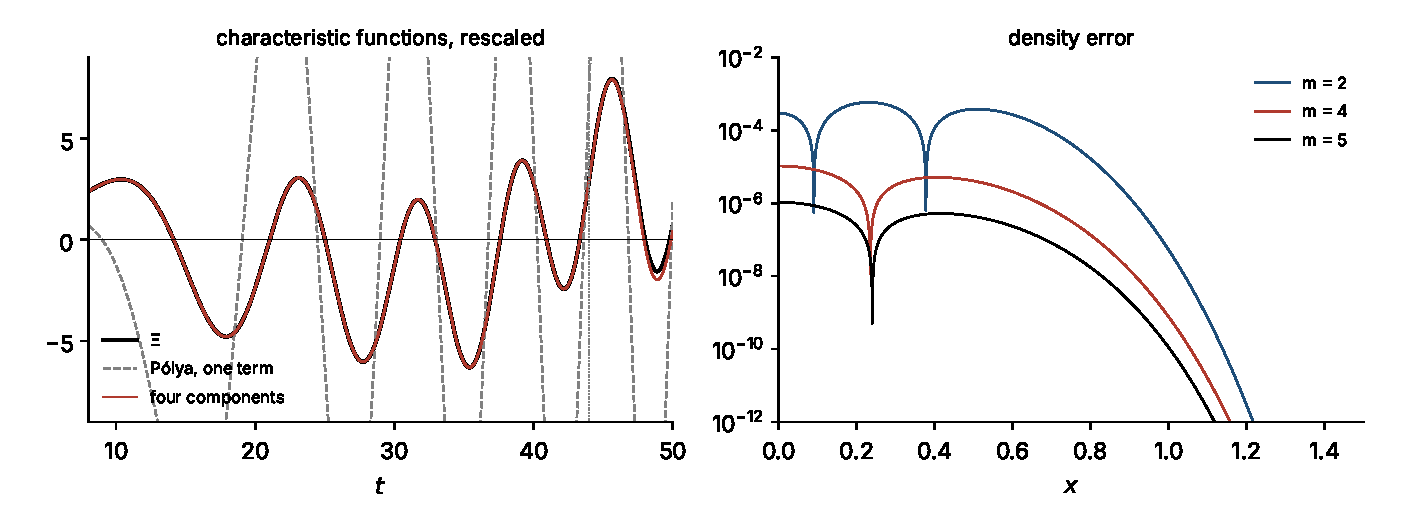
\includegraphics[width=\textwidth]{fig/v3/ap_gigfit.pdf}
\caption{Left: $\Xi$, P\'olya's approximant and the four component fit, rescaled; the window ends at the dotted line. Right: density error for two, four and five components (computed).}\label{ap:fig:gigfit}
\end{figure}
% UNVERIFIED: right panel of ap_gigfit (two and five component errors). The left panel uses the four component fit, reproduced.

\subsection{Longer windows}\label{ap:sec:long}

The window can be extended in double precision if the target is computed in multiple precision, because each factor decays only like $e^{-\pi c_jt/2}$. On $0\le t\le60$, which holds $13$ zeros, the fits of Table~\ref{ap:tab:long} match all thirteen at the rate of about two zeros per component.
\begin{table}[t]
\centering
\small
\begin{tabular}{ccccc}
\toprule
components & $\sum c_j$ & error & zero error & next zeros ($60.83$, $65.11$)\\
\midrule
$6$ & $0.499$ & $0.036$ & $0.013$ & $61.57$, $66.44$\\
$7$ & $0.509$ & $0.025$ & $0.017$ & $60.51$, $65.45$\\
$8$ & $0.491$ & $0.006$ & $0.010$ & $61.60$, $61.71$\\
\bottomrule
\end{tabular}
\caption{Fits on $0\le t\le60$ (computed, double precision, not independently checked). The zero errors are of the order of the grid resolution $0.01$.}\label{ap:tab:long}
\end{table}
% UNVERIFIED: whole of the longer windows table (parameters not printed in the draft); the entry 61.71 for the eight component fit is probably a misprint or a spurious zero.
The errors of the predicted zeros just outside the window are $0.74$ and $1.33$ for six components, $0.32$ and $0.34$ for seven, and $0.77$ and $3.40$ for eight. The last figure uses the entry $61.71$, which lies $0.11$ above the first predicted zero and is probably a misprint or a spurious zero of the fit; without it the errors are $0.3$ to $1.3$. They are worse than at the shorter window. On $0\le t\le76$, with $19$ zeros, our search with nine and eleven components did not find a good fit in ten starts (weighted error above $1$; computed, not verified); we cannot say whether that is a failure of the optimiser or of the family.

\subsection{Who carries which zero}\label{ap:sec:carry}

The zeros of a product are the union of the zeros of its factors, so a fit assigns the zeros of $\zeta$ in the window to its components. The two digit parameters printed with a fit are too coarse to reuse (they give error $0.19$ instead of $5\times10^{-5}$), so Table~\ref{ap:tab:carry} gives a refit with four components, whose parameters we round to two or three digits.
\begin{table}[t]
\centering
\footnotesize
\setlength{\tabcolsep}{4pt}
\begin{tabular}{ccccll}
\toprule
$c$ & $\nu$ & $a$ & zeros carried & next zero of the component & nearest zero of $\zeta$\\
\midrule
$0.095$ & $0.96$ & $0.27$ & $14.135,\ 30.425,\ 43.327$ & $54.92$ & $56.45$\\
$0.151$ & $1.13$ & $1.13$ & two & $49.59$ & $49.77$\\
$0.104$ & $0.52$ & $0.52$ & two & $54.27$ & $52.97$\\
$0.145$ & $0.61$ & $1.37$ & two & $48.02$ & $48.005$\\
\bottomrule
\end{tabular}
\caption{A refit with four components on $0\le t\le44$ (computed). The fit is not unique: the draft's fit had another local minimum, with the split $3,2,2,1$ of the first eight zeros.}\label{ap:tab:carry}
\end{table}
In the refit the first component carries three zeros and the others two each. The last component's second zero falls on $48.02$, against the zero $48.005$ just outside the window. The pattern, not the exact split, is what the fits show: each component is tuned to pass through two or three zeros of $\zeta$ inside the window, and its later zeros, which it cannot choose, miss by $0.02$ to $1.5$. The five component fit shows the same pattern with a different assignment (not verified). This is the split of Proposition~\ref{ap:prop:factor} attempted with GIG spectra. It works for as many zeros as there are free parameters, and no further.

\section{The closure, and what it says}\label{ap:sec:closure}

Let $\overline{\mathcal K}$ be the closure of $\mathcal K$ under convergence in law (it contains the point mass at $0$) and let $\mathcal G$ be the set of characteristic functions of limits in law of finite sums of independent members of $\mathcal K$. By Theorem~\ref{fm:thm:bessel}(i) and Corollary~\ref{fm:cor:coupled}, such sums are ferromagnetic, so by Theorem~\ref{fm:thm:closed} convergence in law of them is locally uniform convergence of the characteristic functions on all of $\mathbb C$, and Hurwitz's theorem applies. Hence $\Xi/\Xi(0)\in\mathcal G$ implies RH. What is $\mathcal G$?

\begin{proposition}[limits of one component]\label{ap:prop:limits}
The closure $\overline{\mathcal K}$ contains
\begin{enumerate}
\item the normal law: $\varphi_{\sigma\sqrt{2a},0,a}(t)\to e^{-\sigma^2t^2/2}$ as $a\to\infty$;
\item the uniform law: $\varphi_{1/L,0,a}(t)\to\sin t/t$ as $a\to0$, with $L=\log(1/a)$;
\item the symmetric two point law: $\varphi_{1/L,\nu,a}(t)\to\cos t$ as $a\to0$, for fixed $\nu>0$.
\end{enumerate}
\end{proposition}

\begin{proof}
For large $a$, $e^{-2a\cosh y}\propto e^{-ay^2(1+o(1))}$, a normal density of variance $1/(2a)$, so $U=c\log W$ with $c=\sigma\sqrt{2a}$ has variance $\sigma^2$. For small $a$, $e^{-2a\cosh y}$ is close to $1$ for $|y|<L-O(1)$ and negligible for $|y|>L+O(1)$. After scaling by $1/L$ the density tends to the uniform density on $(-1,1)$ when $\nu=0$, and when $\nu>0$ the weight $\cosh\nu y$ puts all the mass within $O(1/\nu)$ of $\pm L$.
\end{proof}

Numerically, at $t=2$ (computed): with $a=10^{-300}$ the two small $a$ limits, the second with $\nu=1$, give $0.4554$ and $-0.4146$ against $\sin2/2=0.4546$ and $\cos2=-0.4161$, and the convergence is logarithmic; with $a=1000$ and $\sigma=0.7$ the first gives $0.37537$ against $e^{-2\sigma^2}=0.37531$. So $\mathcal G$ contains every product $e^{-bt^2}\prod_j\cos(a_jt)$, and in particular $\sin t/t=\prod_{j\ge1}\cos(t/2^j)$, together with the components themselves. It is a large class, but a closed one in a restrictive way.

\begin{lemma}[uniform fourth moments]\label{ap:lem:four}
For every component $U$ with characteristic function in $\mathcal K$, $\mathbb E\,U^4\le3(\mathbb E\,U^2)^2$.
\end{lemma}

\begin{proof}
The characteristic function of $U$ is even and has only real zeros, and it is entire of order at most $1$ because the density of $\log W$ decays like $\exp(-ae^{|y|})$. So by Hadamard's theorem it is $\prod_k(1-t^2/t_k^2)$ with $\sum t_k^{-2}<\infty$; there is no Gaussian factor, since $e^{-bt^2}$ has order $2$. Taking logarithms, $\kappa_2(U)=2\sum t_k^{-2}$ and $\kappa_4(U)=-12\sum t_k^{-4}\le0$. Since $U$ is centred, $\mathbb E\,U^4=\kappa_4+3\kappa_2^2\le3(\mathbb E\,U^2)^2$.
\end{proof}

The same proof applies to every even characteristic function with only real zeros that is entire of order at most $1$, as in Corollary~\ref{fm:cor:cum}. On a grid of $a$ from $10^{-12}$ to $10^3$ and $\nu$ in $\{0,\frac12,1,2,5,10,30,100\}$ the ratio $\mathbb E\,U^4/(\mathbb E\,U^2)^2$ lies between $1.00004$ (two point limit) and $2.9995$ (normal limit) (computed).

\begin{theorem}[structure of $\mathcal G$]\label{ap:thm:closure}
Every member of $\mathcal G$ is of the form
\[
e^{-bt^2}\prod_{j\ge1}\varphi_j(t),\qquad b\ge0,\quad\varphi_j\in\overline{\mathcal K},
\]
a normal factor times a finite or countable product of limits of single components. The $\varphi_j$ are characteristic functions of symmetric laws.
\end{theorem}

\begin{proof}
Let $X_n=\sum_jU_{n,j}$, a finite sum of independent components with variances $v_{n,j}$, converge in law to $X$ with characteristic function $\psi$. Write $\varphi_{n,j}$ for the characteristic function of $U_{n,j}$.

\emph{Step 1: the variances are bounded and summable.} By tightness choose $x_0$ with $\mathbb P(|X_n|\ge x_0)<\frac1{24}$ for all $n$. For a symmetric $U$ and an independent $R$, $\mathbb P(|U+R|\ge x)\ge\frac12\mathbb P(|U|\ge x)$, because $2U=(U+R)+(U-R)$ and $|U-R|$ has the law of $|U+R|$. So $\mathbb P(|U_{n,j}|\ge x_0)<\frac1{12}$. By Lemma~\ref{ap:lem:four} and the Paley and Zygmund inequality, $\mathbb P(U^2\ge\frac12\mathbb E U^2)\ge\frac1{12}$, so $v_{n,j}<2x_0^2=:V_0$ for all $n,j$. Next, $\psi(0)=1$, so $\psi\ge\delta>0$ on some $[0,t_0]$, and for large $n$ the product $\prod_j\varphi_{n,j}$ is at least $\delta/2$ there. Each factor has modulus at most $1$, so each $|\varphi_{n,j}|\ge\delta/2$ on $[0,t_0]$, and since $\varphi_{n,j}$ is real and continuous with $\varphi_{n,j}(0)=1$, it is positive on $[0,t_0]$. Hence $\sum_j(1-\varphi_{n,j}(t))\le-\sum_j\log\varphi_{n,j}(t)\le\log(2/\delta)$ on $[0,t_0]$. Averaging over $[0,t_0]$ gives $\sum_j\mathbb E\,h(U_{n,j})\le\log(2/\delta)$ with $h(u)=1-\frac{\sin t_0u}{t_0u}\ge c_0\min(1,u^2)$. The Paley and Zygmund bound again gives $\mathbb E\min(1,U^2)\ge\frac1{12}\min(1,\frac12v)\ge\frac1{24\max(1,V_0)}v$. Hence $\sum_jv_{n,j}\le C'$ for all large $n$, with $C'$ independent of $n$.

\emph{Step 2: the large components converge.} Order the components of $X_n$ by decreasing variance; the $k$th has variance at most $C'/k$. By a diagonal argument, along a subsequence the $k$th component converges in law, for every $k$, to some $U^{(k)}$ with law in $\overline{\mathcal K}$ (possibly a point mass at $0$), and $\mathrm{Var}\,R_{n,k}\to w_k$ for every $k$, where $R_{n,k}$ is the sum of the components after the $k$th. Here $w_k$ is nonincreasing, and by lower semicontinuity of the second moment $\sum_k\mathrm{Var}\,U^{(k)}\le C'$. So $\sum_kU^{(k)}$ converges in $L^2$, and its characteristic function is $\prod_k\varphi^{(k)}$.

\emph{Step 3: the rest is normal.} For centred $U$ with $\mathbb E U^4<\infty$, $|\mathbb E\,e^{itU}-(1-\frac12t^2v)|\le\frac1{24}t^4\mathbb E U^4$ and $|e^{-t^2v/2}-(1-\frac12t^2v)|\le\frac18t^4v^2\le\frac18t^4\mathbb E U^4$. The factors have modulus at most $1$, so the differences of the products are at most the sums of the differences, and by Lemma~\ref{ap:lem:four}
\[
\big|\mathbb E\,e^{itR_{n,k}}-e^{-t^2\mathrm{Var}R_{n,k}/2}\big|\le\frac{t^4}6\sum_{j>k}\mathbb E\,U_{n,j}^4\le\frac{t^4}2\,v_{n,k+1}\sum_jv_{n,j}\le\frac{C'^2t^4}{2(k+1)} .
\]
Now $\psi_n=\prod_{j\le k}\varphi_{n,j}\cdot\mathbb E\,e^{itR_{n,k}}$ with $|\prod_{j\le k}\varphi_{n,j}|\le1$. Letting $n\to\infty$ along the subsequence, $|\psi(t)-\prod_{j\le k}\varphi^{(j)}(t)\,e^{-t^2w_k/2}|\le C'^2t^4/(2(k+1))$. Letting $k\to\infty$, with $w_k\downarrow2b$, gives $\psi=e^{-bt^2}\prod_j\varphi^{(j)}$.
\end{proof}

Step 3 is the Lyapunov central limit estimate with fourth moments. Symmetry and Lemma~\ref{ap:lem:four} are the only properties of the components used, so the theorem holds for products of any family of even characteristic functions with only real zeros of order at most $1$; finite dimensionality of the family plays no role.

Which laws lie in $\overline{\mathcal K}$? Besides the components, it contains by sending the parameters to the boundary the normal laws, the products $\cos(\ell t)\,e^{-\sigma^2t^2/2}$ (from $\nu\to\infty$), and the laws with density proportional to $\cosh(\kappa x/\ell)$ on $(-\ell,\ell)$, $0\le\kappa\le\infty$ (from $a\to0$ with $\nu\log(1/a)\to\kappa$), which interpolate between the uniform and the two point law. The zeros of the last family solve $t\tan(\ell t)=-(\kappa/\ell)\tanh\kappa$ and are asymptotically an arithmetic progression. We have not written out a proof that this list is complete (Problem~\ref{ap:prob:list}). The zero sets that occur are therefore, for the members we know: the sets $\{\tau_n/c\}$ for $\nu=0$; the zero sets of $z\mapsto K_{\nu+iz}(2a)+K_{\nu-iz}(2a)$ for $\nu\ne0$, scaled by $1/c$; arithmetic progressions; and the asymptotically periodic zeros of the truncated $\cosh$ laws. The normal laws have no zeros.

\begin{corollary}[rigidity]\label{ap:cor:rigid}
Suppose $\Xi/\Xi(0)\in\mathcal G$. Then RH holds, $b=0$ in Theorem~\ref{ap:thm:closure}, and $\Xi/\Xi(0)=\prod_j\varphi_j$ with every $\varphi_j\in\overline{\mathcal K}$ nondegenerate. The multiset of ordinates of the zeros of $\zeta$ in the upper half plane is then a disjoint union of the complete zero multisets of the $\varphi_j$, and each $\varphi_j$ equals the canonical product $P_{S_j}$ over its zeros.
\end{corollary}

\begin{proof}
RH holds by the remark before Proposition~\ref{ap:prop:limits}. By Theorem~\ref{ap:thm:closure}, $V$ is the sum of independent variables, a normal variable of variance $2b$ and symmetric variables with laws in $\overline{\mathcal K}$. Each summand is a nondegenerate independent summand of $V$ together with the sum of the others, so by Proposition~\ref{ap:prop:factor} its characteristic function is $P_S$ for an infinite set $S$, and the Gaussian summand has a characteristic function without zeros, whereas $P_S$ with $S$ infinite has infinitely many. So $b=0$. (If the rest of the sum is degenerate there is nothing to prove.) The zeros of the product are the union of the zeros of the factors, counted with multiplicity.
\end{proof}

The converse is not claimed, and it fails for the class $\mathcal G$ as a whole: $e^{-\sigma^2t^2/2}\cos(\ell t)$ lies in $\mathcal G$, by Proposition~\ref{ap:prop:limits}, and is not the canonical product over its zeros, an arithmetic progression. For a member of $\overline{\mathcal K}$ not on the list above we do not know whether it equals the canonical product over its zeros.

The corollary is the answer to the question of the chapter, as a reduction. Approximation by products cannot create in the limit anything that is not already a product. For $\Xi$ to be reached, the ordinates would have to be exactly a disjoint union of complete zero sets of members of $\overline{\mathcal K}$. Under Ingham's hypothesis no progression of three ordinates exists (Problem~\ref{fm:prob:split}), which excludes the arithmetic progressions, but the corollary does not stop there: the sets $\{\tau_n/c\}$ and the zero sets for $\nu\ne0$ remain, and nothing suggests that they sit inside the zeros of $\zeta$. The table of carried zeros shows each fitted spectrum leaving the zeros of $\zeta$ after two or three. So we expect that $\Xi/\Xi(0)\notin\mathcal G$, and then this route gives no proof of RH; the excellent fits are interpolation on a window, and the window cannot be extended to infinity with a fixed type of factor. Everything in this paragraph past the corollary is heuristic, since it depends on Problem~\ref{ap:prob:notG}. Excluding the arithmetic progressions and the sets $\{\tau_n/c\}$ alone would not settle it.

The same reasoning applies to any Hurwitz scheme built from products of a family of even characteristic functions with only real zeros: the limit is an exact product, and the ordinates would have to be a union of the family's zero sets. The only exact product available is Hadamard's, and its factors $1-t^2/\gamma^2$ are not characteristic functions. What remains open is approximation by something other than products, such as sums and mixtures, where reality of zeros is not preserved and has to be proved each time (P\'olya's universal factors, the heat flow), and the splits of Section~\ref{ap:sec:split}, which are exact but use the zeros themselves.

\begin{problem}\label{ap:prob:list}
Prove that the list of $\overline{\mathcal K}$ given after Theorem~\ref{ap:thm:closure} is complete, and determine the zero set of each limit law.
\end{problem}
\begin{problem}\label{ap:prob:iterate}
Prove that the density of Lemma~\ref{ap:lem:remove} is again nonincreasing on $(0,\infty)$ when $f=\Phi/\Xi(0)$, so that the lemma can be iterated, and then prove the conjecture on splits (Remark~\ref{ap:rem:conj}).
\end{problem}
\begin{problem}\label{ap:prob:notG}
Show unconditionally that the multiset of ordinates of the zeros of $\zeta$ is not a disjoint union of complete zero sets of nondegenerate members of $\overline{\mathcal K}$. By Corollary~\ref{ap:cor:rigid} this would prove $\Xi/\Xi(0)\notin\mathcal G$. It needs the zero sets of every member of $\overline{\mathcal K}$, including those with $\nu\ne0$.
\end{problem}
\begin{problem}\label{ap:prob:window}
Settle the window $0\le t\le76$ and beyond with a better optimiser (continuation in $T$, or assigning zeros to components as in Table~\ref{ap:tab:carry}). If $\Xi/\Xi(0)\notin\mathcal G$, as we expect, the corollary predicts that the error at fixed points cannot tend to zero as the window grows; measure how the number of components must grow with $T$.
\end{problem}
\begin{problem}\label{ap:prob:string}
Identify the string of the Wald partner of a GIG component and compare its mass distribution with the string of $H$ computed from the first $1545$ zeros (Section~\ref{c:sec:string}).
\end{problem}
